\chapter{量子情報理論の基礎}

\section{Motivation}
\textcolor{green}{追記が必要な箇所は、緑色の文字で記入。}
\\

\textcolor{red}{わからない点は、赤文字で記入。}
\\

\textcolor{green}{もう一度まとめ直す。}
量子情報の分野では,全体と部分系を分けることで新たの視点や混合状態などが現れる.
そこで,このような全体と部分という視点は,いつも意識しておく必要がある.(CP-mapもPOVMもそれに当たる.)

物理学の統一理論を作りたいが重力だけがまだ統一できていない.具体的には,重力の量子化を行うと高エネルギー領域の量子揺らぎによって起こる紫外発散が頻繁に起こるため量子論として大きな問題が生じる.これは,粒子が点であるとみなすことによって起因するものであると思われている.そこで有限の大きさをもつヒモとして扱う超弦理論は,統一理論の有力な候補として考えられてきた.

ミクロな量子論に問題がある一方,マクロな重力現象にもミステリアスな現象が起こる.統計力学では,識別できない情報量をエントロピーで表す.実は,ブラックホールにも,このエントロピーがあることが知られている.さらに,BHには温度が定義できて熱力学法則も満たすことがわかってきた.(ブラックホール熱力学)

ブラックホールのエントロピー$S_{BH}$は,次の有名なベッケンシュタインホーキングの面積公式
\begin{align}
  S_{BH}=\frac{k_{B}c^3}{4G_{N}\hbar}A
\end{align}
で与えられる.ここで,$A$はBHの表面積である.この式には,様々な物理定数が現れる.重力理論の重力定数,統計力学のボルツマン定数,量子力学のプランク定数が用いられる.言い換えるとこの理論,または公式を本当に理解するためには,これら三つの分野をきちんと融合し量子重力理論を構築する必要がある.

熱力学とブラックホール物理との間には類似性があり,
\begin{center}
内部エネルギーと質量 \\
温度と表面重力\\
エントロピーと面積
\end{center}
それぞれ対応する.これらの対応関係に基づいて,Bekenstein は情報理論の観点 からブラックホールがエントロピーを持つことを示唆した.情報理論では,情報の損失はエントロピーの増加を意味する.ここでは,ある物体がブラックホールに落ち込むことを考える.物体がブ ラックホールに落ち込む前,我々は物体についての情報を知ることができるが,一度,物体がブラッ クホールに落ち込むと,その物体がどういう状態にあるのか我々は物体に対する全ての情報を失うこ とになる.この失われた情報がブラックホールのエントロピーの増加になると考え,ブラックホール が大きなエントロピーを持つことを提案した.そして,そのエントロピーの増加が物体が落ち込むことによって増加するブラックホールの表面積の増加と結び付けた.彼はブラックホールがエントロピーを持つことは示唆したが,温度を持つことまでは提案しなかった.その理由はブラックホールの定義である「どんな粒子の放出を許さない閉鎖的な領域」であることに起因する.ブラックホールが温度を持つ場合,周囲の温度との比較によっては,熱吸収だけではなく,熱放射も説明しなければならない.Bekensteinはブラックホールの放射のメカニズムを説明するまでには至らず,ブラックホー ルが温度を持つとまでは言えなかった.
Bekenstein の論文を受けてHawkingはブラックホールの放射のメカニズムを探し,場の量子論の考察からブラックホール放射のメカニズムを考案した.具体的にはBogoliubov変換を用いて粒子数の期待値がボルツマン分布に従うことを示した,また,熱力学のアナロジーとして温度も定義できる.この特別なブラックホールの温度は,Hawking温度と呼ばれている.Hawkingによりブラックホール放射のメカニズムが明らかとなったため,ブラックホー ル物理と熱力学との間に完全な対応関係を与えることが可能となった.


また,公式からもわかるように,BHのエントロピーは示量変数であるのにも関わらずその体積でなく(通常の統計力学では,エントロピーは体積に比例する)BHの表面積に比例している.(BHのホライズンはほぼ球対称)これは,我々がしる物質とは異なる性質を示しどうしてBHのエントロピーが表面積に比例するのか,あるいはBHのエントロピーとは一体何なのかよくわかっていない.このように,マクロな視点でも解決されていない問題がある.


先ほど述べたように,ブラックホールのエントロピーはBHの中の情報が見れないことによると考えられる.重力を忘れて純粋な量子力学を考えると,量子系の一部が観測できないことによって生じるエントロピーは,エンタングルメントエントロピーと呼ばれる.(量子力学の情報を定式)
そこで,ブラックホールのエントロピーを理解するだ一歩として場の理論におけるエンタングルメントエントロピーを計算する研究が盛んに行われるようになった.(1980年)
(今までのBHのエントロピーの導出は,BHの粒子生成を考えてその粒子数密度から(アナロジー的に)温度を定義してそれを下に,熱的にエントロピーを求めたがそれを量子力学的なアプローチで求めようとする試みである.(これがうまくいくってことは量子力学の中にもう温度という概念が含まれているのか)
\subsection{重力のエントロピーとエンタングルメントエントロピー}
ブラックホールのエントロピーとエンタングルメントエントロピーの類似性は,80年代から議論が進んいる.
重力のエントロピーは,量子力学(場の量子論)のエンタングルメントエントロピーと関係があることを高柳さんたちは示した.これによると,量子場の理論におけるエンタングルメントエントロピーは,一つ次元の高い重力の理論の言葉で書くことができる.


疑問は,重力のエントロピーを知りたかったら,その理論の境界の場の理論のエントロピーを求めれば良さそう。

なので、マルダセナの論文では注意書きがされている.これからやりたいのは,重力のエントロピーを求めたいわけでなない.pureに場の理論における量子相関を求めたいわけである.


\subsection{ホログラフィー原理}
ある時空$\mathcal{M}$における,重力理論は,その境界$\mathcal{\partial M}$における重力理論を含まない場の理論に等価である.
\subsection{AdS/CFT}
反de Sitter時空における量子重力理論は,その境界上の共形場理論に等価である
\subsection{first theses}
Minkowski時空における量子エンタングルメントは,時空の次元によるのものなのか
\section{純粋状態と混合状態}
\subsection{純粋状態におけるエンタングルメント}
純粋状態とは,量子状態$\ket{\phi}$が非自明な確率混合で準備できない状態である.すなわち,Density Matrixが,
\begin{equation}
\label{1}
\rho=\ket{\phi}\bra{\phi}
\end{equation}
の形で与えられる場合である.(\ref{1})式から,純粋状態であれば,
\begin{equation}
\rho^{2}=\rho=1
\end{equation}
が成立する.
\begin{empheqboxed}
  \
  \

  純粋状態$\ket{\phi}$が,エンタングルしてないすなわち,セパラブル(separable)であるときは,
  \begin{equation}
    \label{3}
  \ket{\phi}=\frac{1}{2}(\ket{\uparrow}_{A}+\ket{\downarrow}_{A})(\ket{\uparrow}_{B} +\ket{\downarrow}_{B})=\ket{A}\otimes\ket{B}
  \end{equation}

\end{empheqboxed}

のように,2つの系全体の量子状態が部分系$A,B$の直積として表現できるときである.これに対して,
\begin{empheqboxed}
\
\

エンタングルしている状態としては,

\begin{equation}
    \label{4}
    \ket{\phi_{Bell}}=\frac{1}{\sqrt{2}}(\ket{\uparrow}_{A}\ket{\uparrow}_{B}+\ket{\downarrow}_{A}\ket{\downarrow}_{B})
    \end{equation}
    のように直積で書くことのできない状態である.
\end{empheqboxed}
(\ref{4})式にあげた例は,Bell状態と呼ばれ,
この状態に関するエントロピー,すなわちエンタングルメントエントロピー$S(\rho)$
\begin{empheqboxed}
\

\begin{equation}
\label{defetg}
S(\rho)=-Tr(\rho_{A}\ln \rho_{A})
\end{equation}
\end{empheqboxed}
を最大にし,さらにベルの不等式を最大で破っている場合になっている.ただし,$\rho_A$は,Density MatrixでBについてPartial Traceを取ったもので,
\begin{equation}
\rho_{A}={Tr}_{B}\rho
\end{equation}

で定義される.このように,純粋状態は,片方の状態をPartial Traceをとることでエンタングルメントエントロピーが計算でき,エンタングルしているかどうかを判定することができる.

そのために,混合状態について言及しておく.
\subsection{混合状態におけるエンタングルメントエントロピー}

\textcolor[rgb]{0.4,0.4,0.4}{\begin{align*}
\mathcal{H}_{tot}=\mathcal{H}_{A}\otimes\mathcal{H}_{A}
\end{align*}}


1つの物理系についても,純粋状態と混合状態が定義できる.混合状態と純粋状態では,密度行列の数学的な性質が異なる.例えば,separableな状態である(\ref{3})から構成した密度行列は,
\begin{align}
  \rho^{AB_{p}}=\frac{1}{4}(&\ket{\uparrow}_{A}\ket{\uparrow}_{B}+\ket{\downarrow}_{A}\ket{\uparrow}_{B}+\ket{\uparrow}_{A}\ket{\downarrow}_{B}+\ket{\downarrow}_{A}\ket{\downarrow}_{B})
  (\bra{\uparrow}_{A}\bra{\uparrow}_{B}+\bra{\downarrow}_{A}\bra{\uparrow}_{B}+\bra{\uparrow}_{A}\bra{\downarrow}_{B}+\bra{\downarrow}_{A}\bra{\downarrow}_{B}) \nonumber \\
  =\frac{1}{4}(
&\ket{\uparrow}_{A}\ket{\uparrow}_{B}\bra{\uparrow}_{A}\bra{\uparrow}_{B}+\ket{\downarrow}_{A}\ket{\uparrow}_{B}\bra{\uparrow}_{A}\bra{\uparrow}_{B}+\ket{\uparrow}_{A}\ket{\downarrow}_{B}
\bra{\uparrow}_{A}\bra{\uparrow}_{B}+\ket{\downarrow}_{A}\ket{\downarrow}_{B}\bra{\uparrow}_{A}\bra{\uparrow}_{B}\nonumber \\
&+\ket{\uparrow}_{A}\ket{\uparrow}_{B}\bra{\downarrow}_{A}\bra{\uparrow}_{B}+\ket{\downarrow}_{A}\ket{\uparrow}_{B}\bra{\downarrow}_{A}\bra{\uparrow}_{B}+\ket{\uparrow}_{A}\ket{\downarrow}_{B}
\bra{\downarrow}_{A}\bra{\uparrow}_{B}+\ket{\downarrow}_{A}\ket{\downarrow}_{B}\bra{\downarrow}_{A}\bra{\uparrow}_{B}\nonumber \\
&+\ket{\uparrow}_{A}\ket{\uparrow}_{B}\bra{\uparrow}_{A}\bra{\downarrow}_{B}+\ket{\downarrow}_{A}\ket{\uparrow}_{B}\bra{\uparrow}_{A}\bra{\downarrow}_{B}+\ket{\uparrow}_{A}\ket{\downarrow}_{B}
\bra{\uparrow}_{A}\bra{\downarrow}_{B}+\ket{\downarrow}_{A}\ket{\downarrow}_{B}\bra{\uparrow}_{A}\bra{\downarrow}_{B}\nonumber \\
&+\ket{\uparrow}_{A}\ket{\uparrow}_{B}\bra{\downarrow}_{A}\bra{\downarrow}_{B}+\ket{\downarrow}_{A}\ket{\uparrow}_{B}\bra{\downarrow}_{A}\bra{\downarrow}_{B}+\ket{\uparrow}_{A}\ket{\downarrow}_{B}
\bra{\downarrow}_{A}\bra{\downarrow}_{B}+\ket{\downarrow}_{A}\ket{\downarrow}_{B}\bra{\downarrow}_{A}\bra{\downarrow}_{B}
)
\end{align}
となるが,この式でBに関する物理系をトレースアウトすれば,

\begin{align}
  \rho^{A_{p}}&=\rm{Tr}\rho^{AB_{p}} \\
  &=\frac{1}{2}(
\ket{\uparrow}_{A}\bra{\uparrow}_{A}+\ket{\uparrow}_{A}\bra{\downarrow}_{A}+\ket{\downarrow}_{A}\bra{\uparrow}_{A}+\ket{\downarrow}_{A}\bra{\downarrow}_{A})\\
&=\frac{1}{2}(\ket{\uparrow}_{A}+\ket{\downarrow}_{A})(\bra{\uparrow}_{A}+\bra{\downarrow}_{A})
\end{align}
となり,これは,Aの物理系だけの純粋状態$\bra{\psi}=\frac{1}{\sqrt{2}}(\ket{\uparrow}_{A}+\ket{\downarrow}_{A})$になっていることがわかる.これは,\textbf{separableな状態においてBの物理系ををトレースアウトすれば,Aの純粋状態だけが残る}という非常に当たり前の結果である.また,純粋状態の密度演算子は,二乗すると元に戻るので,
\begin{align}
  \rho^2=\rho,\hspace{2mm}\rm{Tr}\rho^2=1
\end{align}
などの性質がある.次に,entangleな状態から構成される量子状態について考える.


混合状態は,エンタングル状態の2つの物理系から1つをトレースアウトすることで得られる.



混合状態は,純粋状態でない状態すなわち,量子状態$\ket{\phi}$が非自明な確率混合で準備できる状態である.
混合状態では,非自明な確率で様々な量子状態が混合されている状態である,
\begin{equation}
\rho=\sum_{i}p_i\rho_{i}
\end{equation}
\begin{empheqboxed}
  \
  \

  混合状態がセパラブルであるとは,
  \begin{equation}
  \label{30}
  \rho=\sum_{i}p_i\rho^{A}_{i}\otimes\rho^{B}_{i}=\sum_{i}p_i\ket{i}_A\bra{i}_{A}\otimes\ket{i}_B\bra{i}_{B}
  \end{equation}
  と書けるときである.
\end{empheqboxed}
一歩,一般的なDensity Matrixは,
\begin{eqnarray}
\label{40}
\rho=\sum_{ijkl}C_{ijkl}\ket{i}_A\bra{j}_{A}\otimes\ket{k}_B\bra{l}_{B}
\end{eqnarray}
で表される.
\textcolor{green}{以上のことと,fedelty,bell inequolity,traceの値などを次のような表にまとめておくと便利かも.}\footnote{ここでは,2つの物理系のエンタングルメントを考えているが,純粋状態と混合状態は1つの物理系のみで定義できることにも注意したい.また,表記の便宜上純粋状態に関しては,密度行列で書いていないので注意していただきたい.}
{\renewcommand{\arraystretch}{2}
\begin{table}[H]
  \begin{center}
    \begin{tabular}{c|c|c}
       & pure state & mixed state  \\\hline
      separable & $ \ket{\phi}=(\ket{\uparrow}_{A}+\ket{\downarrow}_{A})(\ket{\uparrow}_{B} +\ket{\downarrow}_{B})$ & $\rho=\sum_{i}p_i\rho^{A}_{i}\otimes\rho^{B}_{i}$ \\\hline
      entangle &    $\ket{\phi_{Bell}}=(\ket{\uparrow}_{A}\ket{\uparrow}_{B}+\ket{\downarrow}_{A}\ket{\downarrow}_{B})$  & $\rho=\sum_{i}p_i\rho^{AB}_{i}$
    \end{tabular}
  \end{center}
  \caption{title}
\end{table}}

混合状態では,上と同じ方法を取ってもセパラブル状態でもエンタングルメントエントロピーが$0$とはならいことがある.
そこで,エンタングルメントエントロピーを測度として用いられない.
\begin{empheqboxed}
  \
  \

  pure stateのエンタングルメント判定方法は,次のようにまとめられる.

  \begin{align}
    S(\rho^{A})=0, \hspace{4mm} then\ the\ state\ is\ separable\\
    S(\rho^{A})\neq0, \hspace{4mm} then\ the\ state\ is\ entangle
  \end{align}
\end{empheqboxed}

\section{PPT条件とNegativity}
混合状態や,3つ以上の量子もつれにも適用できる測度としてNegativityがある,\footnote{Negativityが最良の測度であるという意味ではない.}PPT(Positive Partial Transpose)条件は,Density Matrix\ $\rho$に対して,
\begin{eqnarray}
\label{5}
\rho^{T_{A}}
\end{eqnarray}
の固有値が符号によってエンタングルしているか否かを判定する,ここで,上つきの$T_{A}$は,Partial Transpose(部分転置)で,一般的な混合状態(\ref{40})式に適応すると,
\begin{eqnarray}
\label{6}
\rho^{T_{A}}=\sum_{ijkl}C_{ijkl}\ket{j}_A\bra{i}_{A}\otimes\ket{k}_B\bra{l}_{B}
\end{eqnarray}
のように,Aに関してのみ転置を取ることを意味する.(\ref{30})式に適応すれば,
\begin{eqnarray}
\rho^{T_{A}}=\sum_{i}p_{i}\ket{i}_A\bra{i}_{A}\otimes\ket{i}_B\bra{i}_{B}=\rho
\end{eqnarray}
となり,セパラブルな状態であればその固有値は元のDensity Matrixの固有値$1$に等しく正の値となる.
これに対して,セパラブルで書けない,エンタングルしているときは,固有値が負の値になる.\footnote{エンタングルしていても,固有値が正になるときもある.現在までに提案されている様々な測度はエンタングルしているものを全て判定できるわけだはない.}
\subsection{Negativity}
Negativity $N$を(\ref{5})式で定義されたensity Matrixの負の固有値の総和として,
\begin{eqnarray}
N=\sum_{\lambda_{i<0}}|\lambda_i|
\end{eqnarray}
で定義する.ここで,$\lambda$は$\rho^{T_{A}}$の固有値である.さらに,Matrix $X$のTrace Normを次で定義する.
\begin{eqnarray}
||X||=\rm{Tr}\sqrt{X^{\dagger}X}
\end{eqnarray}
すると,$\rho^{T_{A}}$のTrace Normは,
\begin{eqnarray}
\label{7}
||\rho^{T_{A}}||=\sum_{i}|\lambda_{i}|=\sum_{\lambda_{i<0}}|\lambda_i|+\sum_{\lambda_{i<0}}|\lambda_i|
\end{eqnarray}
となる,いま,(\ref{6})式から,
\begin{eqnarray}
\rm{Tr}\rho=\rm{Tr}\rho^{T_{A}}
\end{eqnarray}
であることがわかるので,固有値の総和は,もとのDensity Matrixの固有値の総和$1$に等しく$\sum_{i}\lambda_i$である.したがって,
\begin{eqnarray}
\sum_{\lambda_{i<0}}|\lambda_i|-\sum_{\lambda_{i\leqslant0}}|\lambda_i|=1
\end{eqnarray}
から,
\begin{eqnarray}
 \sum_{\lambda_{i<0}}|\lambda_i|=\sum_{\lambda_{i\leqslant0}}|\lambda_i|+1
\end{eqnarray}
が求まる.これを,(\ref{7})式に代入すれば,
\begin{eqnarray}
||\rho^{T_{A}}||=2\sum_{\lambda_{i\leqslant0}}|\lambda_i|+1
\end{eqnarray}
のように,Density MatrixとNegativityに関係が得られた.さらに,
\begin{eqnarray}
L(N)=\log||\rho^{T_{A}}||=\log(2N+1)
\end{eqnarray}
のように,対数を取れば,エンタングルメントエントロピーと同様の加法性などのせいなどの性質を満たす.この値をLogarithmic negativityという.
\section{量子力学と統計力学エントロピー}
\subsection{カノニカル・アンサンブル}
熱浴の中にある閉じた系で,ある微視的状態$n$が実現する確率は,
\begin{equation}
  \label{22}
  p_n=\frac{e^{-\beta E_n}}{\sum_{k}e^{-\beta E_k}}
\end{equation}
となる.このようなアンサンブル (分布) をカノニカル・アンサンブル(canonical ensemble,正準集団) あるいはカノニカル分布 (canonical distribution) と呼ぶ.(\ref{22})式の分母に含まれる和は,分配関数のと呼ばれ
\begin{equation}
  Z=\sum_{n}e^{-\beta E_n}
\end{equation}
で定義される,また,ヘルムホルツの自由エネルギー$F$と分配関数の関係は,
\begin{equation}
  F=-\frac{1}{\beta}\log Z
\end{equation}
の関係がある.はじめにこの関係について導出する.

-----村上さんのをみよ------



次に,統計に力学におけるエントロピーを確認する,
統計力学では,エントロピーはヘルムホルツの自由エネルギー$F$を用いて,
\begin{equation}
  S=\frac{1}{T}(E-F)
\end{equation}
で表すことができる.まずこれを示し,量子力学におけるエントロピーと統計力学におけるエントロピーの関係性について議論する.
混合状態における温度$T=\frac{1}{T}$のカノニカル分布の密度行列は,
\begin{eqnarray}
\label{25}
\rho_{tot}=\frac{e^{-\beta \mathcal{H}}}{Z}
\end{eqnarray}
で与えられる.系のエンエトロピーを統計力学に従って計算すると,
\begin{eqnarray}
S_{tot}&=&-\frac{\partial F}{\partial T}=\beta^2\frac{\partial F}{\partial \beta} \\
\label{27}
&=&\frac{1}{Z}(\rm{Tr}[\beta\mathcal{H}e^{-\beta \mathcal{H}}]+Z\log Z) \\
\label{28}
&=&\beta(E-F)
\end{eqnarray}
となり熱力学的なエントロピーと自由エネルギーの関係,
\begin{eqnarray}
F=E-ST
\end{eqnarray}
を得る.
また,(\ref{25})を用いて,(\ref{27})式を変形すると,
\begin{equation}
  S_{tot}=\frac{1}{Z}\biggl(\rm{Tr}[-\rho_{tot}Z\log(\rho_{tot}Z)]+Z\log Z\biggr)
\end{equation}
さらに,
\begin{equation}
  \rm{Tr}(\rho_{tot})=1
\end{equation}
に注意すれば,熱力学的なエントロピー(\ref{28})式は,
\begin{equation}
  S_{tot}=-\rm{Tr}(\rho_{tot}\log\rho_{tot})
\end{equation}と書き換えられる.これは,行列$\rho_{tot}$に関するフォンノイマンエントロピーである.従って,混合状態が統計力学の分布に従うとき,熱力学的なエントロピーは,フォンノイマンエントロピーに一致する.すなわち,統計力学における熱力学的なエントロピーは量子力学の密度行列の気泡を用いるると,フォンノイマンエントロピーとして,簡潔に記述できる.

\section{Tsallis Entropy(ツァリス エントロピー)}
Tsallis Entropyは,Von Neumann Entropyの拡張として,
\begin{align}
  S_{n}=\frac{1-\rm{Tr}\rho^n}{n-1}=\frac{1-\sum_{i}\lambda_{i}^n}{n-1}
\end{align}
で定義される.二個目の等号への式変形は,トレースの性質を用いて密度行列を対角化することによって得られる.このTsallis Entropyは,$n=1$の極限でVon Neumann Entropyに一致する.それをはじめに示す.
(proof)

今,固有値$\lambda_{i}^{n}$は,テイラー展開の公式.
\begin{align}
  e^{x}=\sum_{k=0}^{\infty}\frac{1}{k!}x^{k}
\end{align}
を用いて,
\begin{align}
  \lambda_{i}^{n}=\lambda_{i}\lambda_{i}^{n-1}=\lambda_{i}e^{(n-1)\log \lambda_{i}}=\lambda_{i}\sum_{k=0}\frac{1}{k!}((n-1)\log \lambda_{i})^{k}
\end{align}
となるので,Tsallis Entoropyは,
\begin{align}
S_{n}&=\frac{1}{n-1}\biggl\{1-\sum_{i}\lambda_{i}\sum_{k=0}\frac{1}{k!}((n-1)\log \lambda_{i})^{k}\biggr\}\\
&=\frac{1}{n-1}\biggl\{1-\sum_{i}\lambda_{i}-\sum_{i}\lambda_{i}\sum_{k=1}\frac{1}{k!}((n-1)\log \lambda_{i})^{k}\biggr\}\\
&=-\sum_{i}\lambda_{i}\sum_{k=1}\frac{1}{k!}(n-1)^{k-1}(\log \lambda_{i})^{k}
\end{align}
のように変形できる.二行目から三行目の変形は,全ての確率の総和が$\sum_{i}\lambda_{i}=1$になることを利用している.最後に,この式で,$n \to 1$の狂言をとると.総和のうち$k=1$の項のみが有限の値になり,あとは全て0になるので,
\begin{align}
  S_{1}=\lim_{n \to 1}S_{n}&=-\lim_{n \to 1}\sum_{i}\lambda_{i}\sum_{k=1}\frac{1}{k!}(n-1)^{k-1}(\log \lambda_{i})^{k}\\
  &=-\sum_{i}\lambda_{i}\sum_{k=1}\frac{1}{k!}(1-1)^{k-1}(\log \lambda_{i})^{k}\\
  &=-\sum_{i}\lambda_{i}\log \lambda_{i}
\end{align}
を得る.これは,まさに,Von Neumann Entoropyである.

一方,l'Hospitalの定理を用いると.Tsallis Entropyは,
\begin{align}
  \label{1.50}
  \lim_{n \to 1}S_{n}&=\lim_{n \to 1}\frac{1-\mathrm{Tr}\rho^n}{n-1}
  =-\lim_{n \to 1}\frac{\partial}{\partial n}(\mathrm{Tr}\rho^n)\\
  &=\lim_{n \to 1}\frac{-\dfrac{\partial}{\partial n}(\mathrm{Tr}\rho^n)}{\mathrm{Tr}\rho^{n}}
  \label{1.51}
  =-\lim_{n \to 1}\frac{\partial}{\partial n}(\log\mathrm{Tr}\rho^{n})
\end{align}
のように,二通りでVon Neumann Entropyが表現できる.二行目の式変形でも,全確率が$1$になること,すなわち$\lim_{n \to 1}\mathrm{Tr}\rho^n=1$を用いた.
\begin{align}
  \lim_{n \to 1}\mathrm{Tr}\rho^n=\lim_{n \to 1}\sum_{i}\lambda_{i}^n=\sum_{i}\lambda_{i}=1
\end{align}
これは,\ref{1.50}式から\ref{1.51}式の分子はエントロピーに一致する値なので収束するため,分母に$1$に収束する$\lim_{n \to 1}\mathrm{Tr}\rho^n=1$を付け加えたことになる.(分子が収束するので分母分子で極限がすぐに取れる.)

以上より,エントロピーは,
\begin{empheqboxed}

  \begin{align}
    \label{replica}
    S_{1}=-\lim_{n \to 1}\frac{\partial}{\partial n}(\mathrm{Tr}\rho^n)=-\lim_{n \to 1}\frac{\partial}{\partial n}(\log\mathrm{Tr}\rho^{n})
  \end{align}

\end{empheqboxed}
のようにかける.この式で,$n$は,replica数と呼ばれ,場の理論や,スオイングラスなどにおけるエンロピーを求める時によく用いられる.

\begin{align}
  \lim_{n \to 1}(1-n\frac{\partial}{\partial n})\log \mathrm{Tr}\rho^{n}
\end{align}
\textcolor{red}{の導出を行う}
\section{場の理論におけるEntanglement Entropy\cite{15}\cite{16}\cite{17}\cite{18}}
\subsection{replica法(Calabrese-Cardyの方法)}
次に,場の理論におけるエンタングルメントエントロピーを求める方法であるreplica法についてのべる.以下の議論は,簡単のために二次元で考える.
上の議論で,量子状態は$\ket{\uparrow}$などは,その状態のエネルギーによって特徴ずけられていた.また.またそれらの状態の和として波動関数または,Desity Matrixが定義された.一方,場の理論での量子状態および波動関数は,場$\phi$によって定まるという特徴があった.そこで場の理論におけるエンタングルメントエントロピーを求める時.トレースは,エネルギー固有状態での和ではなく全ての場の配位によって和を取れば良い.さらに,我々が考えたいのは,真空におけるエンタングルメントエントロピーであったので,次のような波動関数$\psi[\phi(x_{1})]$を考えれば良い.[\textcolor{green}{九後}]


\footnote{このような波動関数を考える理由についてもっと詳しく書く.場の理論における真空のエンタングルメントエントロピーを求めるために,$\rho=\ket{0}\bra{0}$を考えてこのトレースを計算することがここでやりたいことである.しかし,場の理論における真空は,Lagrangianを定義することによって定まる.すなわち.このままトレースを計算することは,lagraginaの情報を与えていないので難しい.そこで,はじめに場の配位が与えられた時の波動関数を計算し.それの和について考える.具体的には,以下の要領.
\begin{align}
  \ket{\psi}=\frac{1}{\sqrt{3}}\ket{1}+\frac{2}{\sqrt{6}}\ket{2}
\end{align}
のトレースは,
\begin{align}
  \mathrm{Tr}\rho=\frac{1}{3}\braket{1|1}+\frac{2}{3}\braket{2|2}
\end{align}
である.一方,あるエネルギー固有状態$\ket{n}$に対する波動関数
\begin{align}
  \psi(n)=\braket{n|\psi}=\frac{1}{\sqrt{3}}\braket{n|1}+\frac{2}{\sqrt{6}}\braket{n|2}
\end{align}について考えよう.
この波動関数から作られるdesity matrixに相当する$\rho_{\psi(n)\psi^{*}(n)}$は,
\begin{align}
  \rho_{\psi(n)\psi(n)^{*}}&=(\frac{1}{\sqrt{3}}\braket{n|1}+\frac{2}{\sqrt{6}}\braket{n|2})(\frac{1}{\sqrt{3}}\braket{1|n}+\frac{2}{\sqrt{6}}\braket{2|n})\\
  &=\frac{1}{3}\braket{n|1}\braket{1|n}+\frac{\sqrt{2}}{3}\braket{n|1}\braket{2|n}
  +\frac{\sqrt{2}}{3}\braket{n|2}\braket{1|n}+\frac{2}{3}\braket{n|2}\braket{2|n}
\end{align}となる.ブラケットの積の順番は入れ替えられることに注意して最後に,$n$に関する和を取と,
\begin{align}
  \sum_{n}\rho_{\psi(n)\psi(n)^{*}}&=  \sum_{n}\biggl(\frac{1}{3}\braket{1|n}\braket{n|1}+\frac{\sqrt{2}}{3}\braket{2|n}\braket{n|1}
  +\frac{\sqrt{2}}{3}\braket{1|n}\braket{n|2}+\frac{2}{3}\braket{2|n}\braket{n|2}\biggr)\\
  &=\frac{1}{3}\braket{1|1}+\frac{2}{3}\braket{2|2}
\end{align}
を得る.これは上の結果と同じである.以下では$\ket{n}$の役割を場$\phi(x)$に置き換えて同じことを実行する.}
\begin{align}
  \psi[\phi(x_{1})]=\braket{\phi(x_1)|0}
\end{align}
この値は,場の理論の経路積分表示によって表すことができる.時刻$x_0=X_0$の時の波動関数は,場の配位$\phi(x_0,x_1)$の汎関数である.
理論に時間方向の並進対称性があれば,$X_0=0$と置ける.\footnote{ここで,理論に時間並進対称性がある仮定した.}(あとで述べるが,ここでいう$x_0$はwick rotation後の座標である.)このことに注意すれば,波動関数が経路積分で表示できる.その前に,量子力学の例をもう一度振り返ることで,見通しよく計算を進める.

量子力学における,時刻$t_i$で位置$q_i$にいる状態から,時刻$t_f$で位置$q_f$にいる状態への遷移振幅は,経路積分を用いいて,
\begin{align}
  \braket{q_f,t_f|q_i,t_i}&=\int^{q(t_f)=q_f}_{q(t_i)=q_i}Dq \exp(i\int^{t_f}_{t_i}dt\mathcal{L})\\
  &=\int^{q(\tau_f)=q_f}_{q(\tau_i)=q_i}Dq \exp(-\int^{\tau_f}_{\tau_i}d\tau\mathcal{L}_{E})
\end{align}
とかける.一行目から二行目への変形は,$\tau=it$のwick rotationを行なった.対応は,$dt=-id\tau$,$\tau_i=it_i$,$\tau_f=it_f$である.また,指数の中のマイナス符号は,lagragianから出てきたものである.
また,積分測度は,次のように定めた.
\begin{align}
  Dq=\prod_{a=1}^{n}\prod_{j=1}^{N}dq_{j}^a=\prod_{j_1=1}^{N_1}dq_{j_1}^1\prod_{j_2=1}^{N_2}dq_{j}^2\cdots
\end{align}
$a$は,次元の自由度で二次元では$dq_{j}^1 dq_{j}^2$の積の総乗になる.また$j$は,座標の総乗である.
この経路積分の表式のanalogyから,時刻$x_0=0$における,場の配位が$\phi(x_1)$で与えられる基底状態(真空)の波動関数は,
\begin{align}
  \psi[\prod_{x_1}\phi(x_{1})]&=\braket{\underbrace{\prod_{x_1}\phi(x_1)}_{x_{0f}=0}|0} \\
  \label{a}
  &=\lim_{it_i\to -\infty}\braket{\phi(x_1)|e^{-i\mathcal
  {H}(t_f-t_i)}|\psi}\\
  &=\lim_{x_{0i}\to -\infty}\frac{1}{\sqrt{Z}} \int D\phi \exp\biggl(-\int^{0}_{x_{0i}}dx_0\int dx_1\mathcal{L}\biggr)\times\delta(\phi(x_{0f}=0,x_1)-\phi(x_1))\\
  \label{b}
  &=\frac{1}{\sqrt{Z}} \int D\phi \exp\biggl(-\int^{0}_{-\infty}dx_0\int dx_1\mathcal{L}\biggr)\times\delta[\phi(x_{0f}=0,x_1)-\phi(x_1)]
\end{align}
から求められる.ここで,一行目から二行目への変形は,$t_i\to -\infty$で波動関数$\ket{\psi}$が基底状態(真空)になることを用いた.\footnote{実際,$\lim_{it_i\to -\infty}=\lim_{x_{0i}\to -\infty}$で波動関数$\ket{\psi}$が基底状態(真空)になることを確かめる.波動関数$\ket{\psi}$がハミルトニアンの固有状態で展開できるとすると,
\begin{align}
  \ket{\psi}=\sum_{i}c_{i}\ket{i}
\end{align}
であるので,これを代入すれば,
\begin{align}
  \lim_{x_{0i}\to -\infty}\braket{\phi(x_1)|e^{-i\mathcal
  {H}(t_f-t_i)}|\psi}&=\lim_{x_{0i}\to -\infty}\sum_{i}c_{i}\braket{\phi(x_1)|e^{\mathcal
  {H}(x_{0i})}|i}\\
  &=\lim_{x_{0i}\to -\infty}e^{E_0x_0}\sum_{i}c_{i}e^{(E_i-E_0)x_0}\braket{\phi(x_1)|i}
\end{align}
を得る.初めに,wick rotationした時間座標$it=x_0$をもいて書き直しをした.さらに,一行目から二行目への変形は,$x_{0f}=0$と取れることと,$\ket{i}$がハミルトニアンの固有状態であることを用いた.今,$E_0$はハミルトニアンの基底状態のエネルギーであるので,$E_{i}-E_0>0$であるので,$\lim_{x_{0i} \to -\infty}e^{(E_i-E_0)x_0}=0$である.したがって,基底状態のエネルギー$E_0$を$E_0=0$のように定めれば,
\begin{align}
  \lim_{x_{0i}\to -\infty}\braket{\phi(x_1)|e^{-i\mathcal
  {H}(t_f-t_i)}|\psi}&=\lim_{x_{0i}\to -\infty}c_0e^{E_0x_0}\braket{\phi(x_1)|0}\\
  &=c_0\braket{\phi(x_1)|0}
\end{align}
となる.したがって$\lim_{it_i\to -\infty}\braket{\phi(x_1)|e^{-i\mathcal
{H}(t_f-t_i)}|\psi}$は$\braket{\phi(x_1)|0}$に位相を除いて一致することが確かめられた.}
さらに,$\prod_{x_1}\phi(x_1)$は,まとめて$\phi(x_1)$と略記した.以降,この省略に注意して議論をする.\footnote{汎関数の表記に仕方なのでこのように表記するのが本来正しいだろう.}二行目から三行目への変形は,量子力学の経路積分表示を参考にした.(対応は,$t\rightarrow t,x$と$x\rightarrow \phi$である.)
$Z$は,規格化因子で次で定義される分配関数である.
\begin{align}
  Z=\int D\phi e^{-S[\phi(x_0,x_1)]}
\end{align}
\textbf{$\ket{\psi}$は,真空状態を含む任意の波動関数であるので,経路積分表示における境界条件は$x_{oi}\to -\infty$を取ることを行えば良い.このためデルタ関数は,最終状態の$\phi(x_{0f},x_1)$のみだけが書かれている.}ここで,注意したいことは,このデルタ関数も総乗である,すなわち,
$\delta(\phi(x_{0f}=0,x_1)-\phi(x_1))=\prod_{x_1}\delta(\phi(x_{0f}=0,x_1)-\phi(x_1))$の意味で使われている. したがって,
\begin{align}
  \int\prod_{x_1}[d^{\prime}\phi(x_1)]G[\phi(x_1)]\times\delta[\phi(x_1)-\bar{\phi}(x_1)]=G[\bar\phi(x_1)]
\end{align}
これは,積分測度の中に総乗が隠れているからである.すなわち.
\begin{align}
  D\phi(x_1)\propto \prod_{x_1}d\phi(x_1)
\end{align}
であるからである.さらに,デルタ関数の中に含まれる$\phi(x)$についてもコメントをしておく.引数の初めの$\phi(0,x_1)$は,積分される場の値である.一方で,引数の2番目の$\phi(x_1)$は,初めに与えた場$\phi(x_1)$である.したがって,この値は一つの値に固定されている.また汎関数のデルタ関数は,主に次の意味で使われている.
\begin{eqnarray}
\delta[\phi(x_1)-\bar{\phi}(x_1)]=\prod_{x_1}\delta(\phi(x_1)-\bar{\phi}(x_1))
\end{eqnarray}

次にこの波動関数の複素共役な波動関数について考える.式(\ref{a})を参考にすれば,指数関数の肩の値は,$it \rightarrow -it$と変えればいいので,これを$x_0$の言葉で書き換えると,複素共役では$x_0 \rightarrow -x_0$と対応付くことに注意する.すなわち,上のやった$x_{0i}\to -\infty$で計算するトリックは,$x_{0i}\to \infty$とすれば良い.よって,
\begin{align}
  \psi^{*}[\phi(x_{1})]=\frac{1}{\sqrt{Z}} \int D\phi \exp\biggl(-\int_{0}^{\infty}dx_0\int dx_1\mathcal{L}\biggr)\times\delta[\phi(0,x_1)-\phi(x_1)]
\end{align}
とかける.(微小量$dx_0$も$-dx_0$になることに注意した.)このときの積分測度は,(\ref{b})とは異なり,
\begin{align}
  D\phi\propto \prod_{0<x_0<\infty}\prod_{x_1}d\phi(x_0,x_1)
\end{align}
で定義される.以上をまとめると,以下のようになる.

\begin{empheqboxed}

\begin{align}
\label{wave1}
  \psi[\phi(x_{1})]&=\frac{1}{\sqrt{Z}} \int \prod_{-\infty<x_0<0}\prod_{x_1}d^{\prime}\phi(x_0,x_1) \exp\biggl(-\int_{0}^{\infty}dx_0\int dx_1\mathcal{L}\biggr)\times\delta[\phi(-\epsilon,x_1)-\phi(x_1)] \\
  \label{wave2}
  \psi^{*}[\phi(x_{1})]&=\frac{1}{\sqrt{Z}} \int \prod_{0<x_0<\infty}\prod_{x_1}d^{\prime}\phi(x_0,x_1) \exp\biggl(-\int^{0}_{-\infty}dx_0\int dx_1\mathcal{L}\biggr)\times\delta[\phi(+\epsilon,x_1)-\phi(x_1)]
\end{align}

\end{empheqboxed}

ここで,デルタ関数の中身を上の議論よりも正確に書いた.複素共役を取る前の波動関数の$x_0$に関する積分区間は,負の値であるので,それに対応する$0$の値は府側から近づけた値であるので$-\epsilon$と書いた.同様にして,複素共役をとった波動関数の$x_0$に関する積分区間は,正であるので$+\epsilon$と書いた.

最後に波動関数の規格化因子について確認しておく.量子力学では,ノルムの総和が1になるよう規格化をした.上の求めた波動関数のノルムの総和は,同様にして,
\begin{align}
  \sum_{\phi(x_1)}\braket{\phi(x_1)|0}\braket{0|\phi(x_1)}&=\int\prod_{x_1}[d\phi(x_1)]\psi[\phi(x_{1})]\psi^{*}[\phi(x_{1})] \\
  &=\int\prod_{x_1}[d\phi(x_1)]\frac{1}{Z}\prod_{-\infty<x_0<\infty}\prod_{x_1}d^{\prime}\phi(x_0,x_1) \exp\biggl(-\int^{\infty}_{-\infty}dx_0\int dx_1\mathcal{L}\biggr)\delta[\phi(0,x_1)-\phi(x_1)]\\
  &=\frac{1}{Z}\int D\phi(x_0,x_1) \exp\biggl(-\int^{\infty}_{-\infty}dx_0\int dx_1\mathcal{L}\biggr)\\
  &=\frac{1}{Z}Z=1
\end{align}
となり,1になる,すなわち$\frac{1}{Z}$は規格化因子となっていることがわかる.密度演算子の視点で考えると,これは$\mathrm{Tr}\rho=1$に対応する.ここで確認しておくべきことは,場の理論の場合は,traceをとるときに全ての位置$x$における全ての場の配位を足し上げているところである.

最後に,波動関数から作られる密度行列について考える.全体系の密度行列は,二つの境界条件によって,
\begin{align}
  [\rho_{tot}]_{\phi_{-}(x_1)\phi_{+}(x_1^{\prime})}=\Psi[\phi(x_1)]\Psi[\phi(x_1)]
\end{align}
と書くことができる.ここで,密度行列の足は,時刻$t,x_0=0$における場の配位$\phi(x_1)$の関数全体ので張られる関数空間である.$\phi_{+},\phi_(-)$と書いている理由は,$x_0=\pm\epsilon$それぞれの時刻における場という意味であり,これらの配位は,積分で全ての配位を足し合わせるので,同じ値を走る,そのため行列の足としてきちんと昨日している.さらに領域Bに関する部分をトレースアウトすれば,Aに関する縮約密度行列は,
\begin{align}
  [\rho_{A}]_{\phi_A(x_-)\phi_A(x_+)}=\frac{1}{Z}&\int\prod_{x_1 \in B}[D\phi(x_1)]\int D\phi \exp\biggl(-\int_{-\infty}^{\infty}dx_0\int dx_1\mathcal{L}\biggr)\nonumber \\
  &\qquad \times\delta[\phi(-\epsilon,x_1)-\phi_{A}(x_{1-})]\delta[\phi(+\epsilon,x_1)-\phi_{A}(x_{1+})] \\
  =\frac{1}{Z}&\int D\phi \exp\biggl(-\int_{-\infty}^{\infty}dx_0\int dx_1\mathcal{L}\biggr)\\
  &\qquad
  \times\prod_{x_1\in A}\delta(\phi(-\epsilon,x_1)-\phi_{A}(x_{1-}))\delta(\phi(+\epsilon,x_1)-\phi_{A}(x_{1-}))
\end{align}
のように,Aの領域だけのデルタ関数が残る.
\subsubsection{Note}

\hrulefill

Bの領域でのトレース

\hrulefill
最終的に求めたいものは,これの$n$コピーしたもので,全体のトレースをとれば領域Aのエンタングルメントエントロピーが求められることになる.\textbf{先ほども注意したように,境界条件になる場の配位$\phi_{A}(x)$は,全ての値をとりうるのでこれがちょうど行列の足になっている.}

したがって,$n$乗した密度行列は,行列の計算方法から
\begin{align}
  \mathrm{Tr}\rho_{A}^{n}=\biggl(\prod^{n}_{j}[D\phi_{j}]\biggr)[\rho_{A}]_{\phi_1\phi_2}[\rho_{A}]_{\phi_2\phi_3}+\cdots+[\rho_{A}]_{\phi_n\phi_1}
\end{align}
と表すことができる.traceをとるので初めて終わりの足も揃っていることに注意したい.この表式は.次のようにも解釈できる.時間と空間を$z=x_1+ix_0 \in \mathcal{C}$と表すと,$\mathrm{Tr}(\rho_A)^n$は,$n$枚の複素平面をスリットのところで連結したリーマン面($\mathrm{R}_n$)上に定義された分配関数と考えられる,実際,traceをとるので,異なる面の境界条件を,$k=1,2,\cdots,n$
\begin{align}
  \label{harituke}
  \phi_{A}^{(k)}(\tau=-\epsilon,x_1)=\phi_{A}^{(k-1)}(\tau=+\epsilon,x_1)\\
  \label{harituke1}
  \phi_{A}^{(1)}(\tau=-\epsilon,x_1)=\phi_{A}^{(n)}(\tau=+\epsilon,x_1)
\end{align}
で与える.もしくは,
\begin{align}
  \phi_{A}^{(k)}(e^{2\pi i}(w-u))=\phi_{A}^{(k+1)}(w-u)\\
  \phi_{A}^{(k)}(e^{2\pi i}(w-v))=\phi_{A}^{(k-1)}(w-v)
\end{align}
で与えことと同じになる.この条件はくるっと一周回れば上のシートに行くことを意味する,実際,(\ref{harituke}),(\ref{harituke1})式で与えれる条件は,これを意味する.図的には,図\ref{replica00}を参考すると良い.\textcolor{red}{ここら辺がしっかり理解できていない$w$とは何か}
\begin{figure}[H]
\begin{center}
  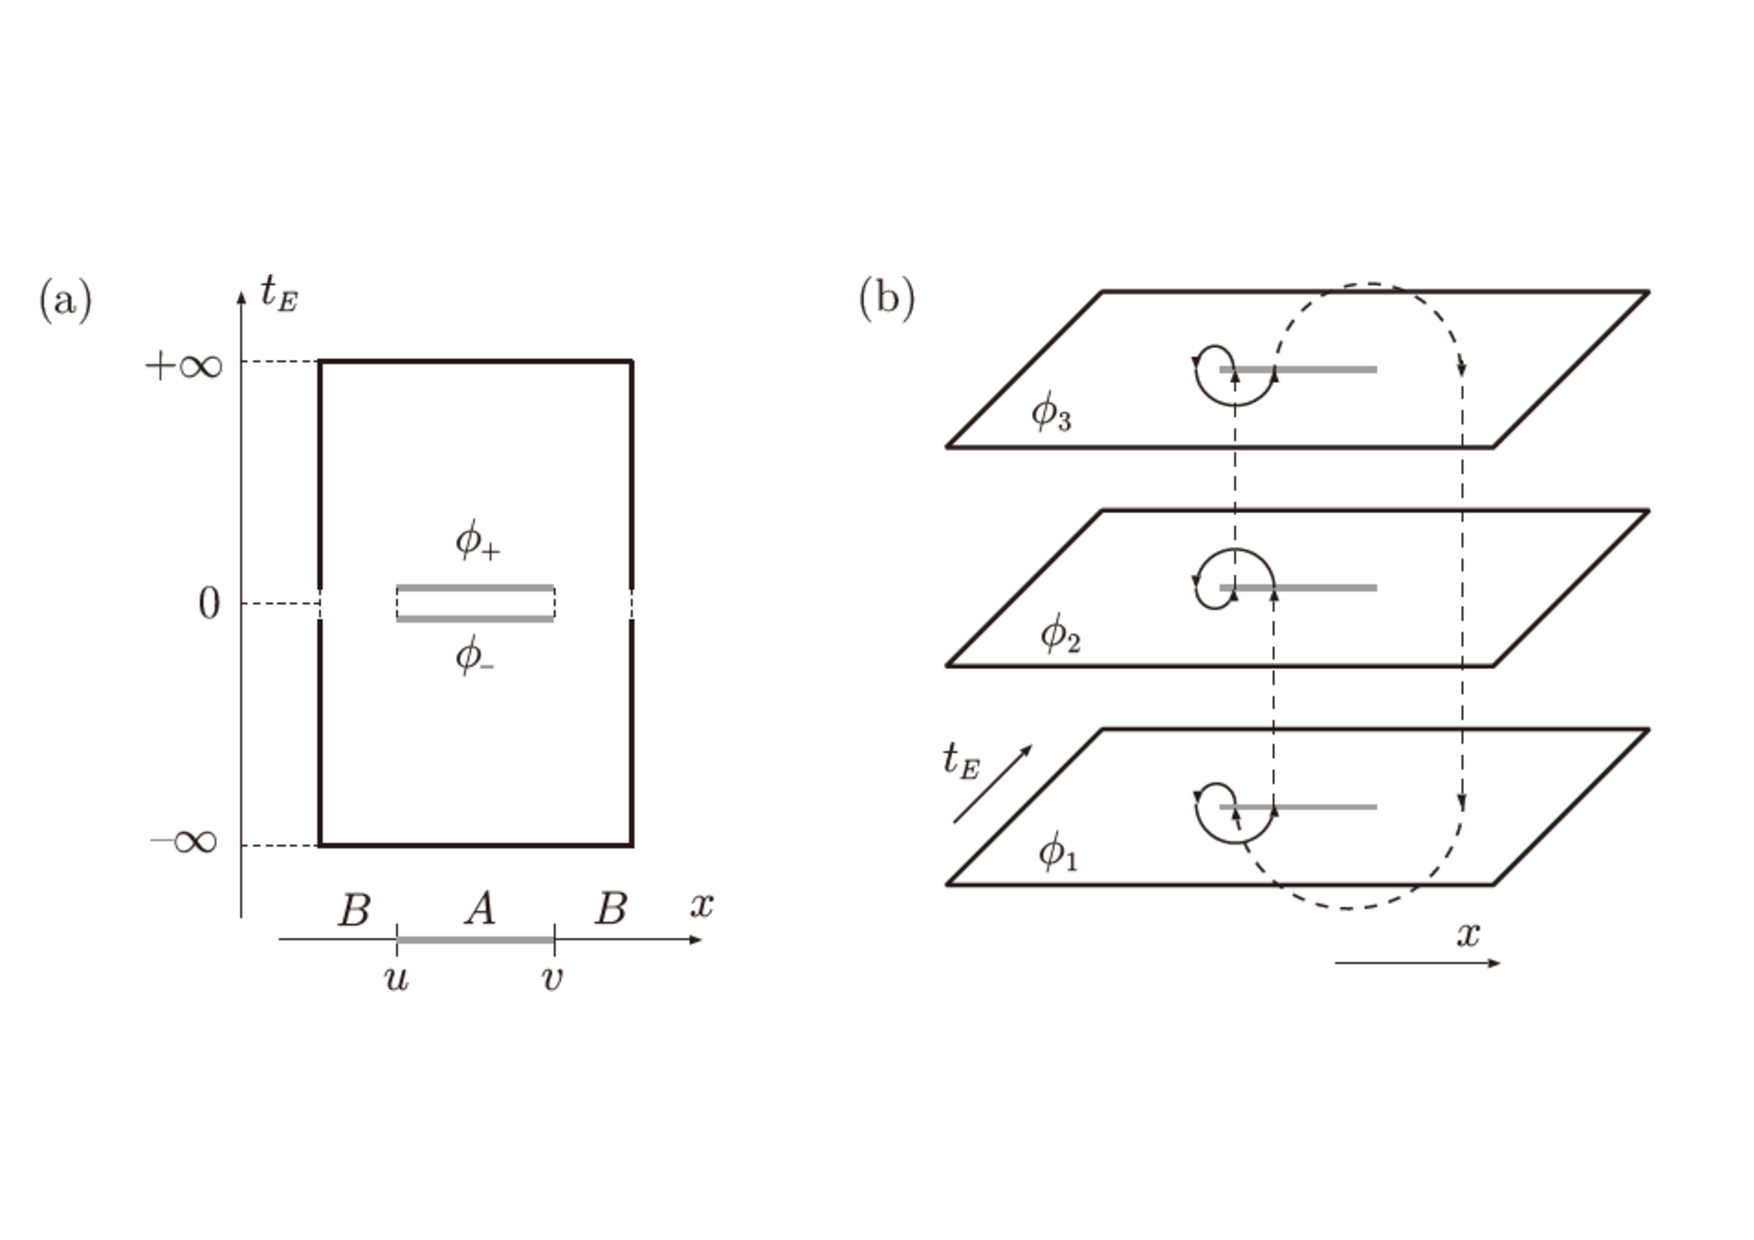
\includegraphics[width=12cm,angle=0]{replica.pdf}
     \caption{}
    \label{replica00}
\end{center}
\end{figure}

これらのことを求めると,$\mathrm{Tr}(\rho_A)^n$は,
\begin{align}
  \mathrm{Tr}\rho_{A}^{n}=&\biggl(\prod^{n}_{j}[D\phi_{j}]\biggr)[\rho_{A}]_{\phi_1\phi_2}[\rho_{A}]_{\phi_2\phi_3}+\cdots+[\rho_{A}]_{\phi_n\phi_1}\\
  -&\frac{1}{(Z_1)^n}\int_{\mathcal{R}_n}\mathcal{D}\phi e^{-\int dx_0dx_1\mathcal{L}^{n}}
\end{align}
と表すことができる.あとは,この値を計算することによって,領域Aにおけるエンタングルメントエントロピーを求めることができる.

\newpage

\subsubsection{Note}

\hrulefill

Q,Mの波動関数は$\phi(x)$で,これは位置$x$における情報しか持っていない.一方,場の理論の波動関数$\psi[\phi(x)]$は汎関数で表されて,初めから場全体の情報が含まれている(全ての$x$の情報).そのため場の理論の波動関数は,エンタングルメントなどの物理量を求める時に必要なdata setが初めから用意されていて,量子力学の時のように直積で後から加える必要がない.

\hrulefill

\subsubsection{エンタングルメントエントロピーの具体的な計算}
この節では,具体的なエンタングルメントエントロピーの計算を行う.簡単のために平坦な場のスカラー場について計算する.そこで,作用は,
\begin{align}
  S[\phi]=&\int dx_0d^dx\biggl[\frac{1}{2}(\partial_{x_0}\phi)^2+\frac{1}{2}(\partial_{x_1}\phi)^2+\frac{m^2}{2}\phi^2\biggr]\\
  =&\frac{1}{2}\int dx^{d+1}\phi(x)[\Delta+m^2]\phi(x)
\end{align}
部分積分を行った.
ここで,
\begin{align}
  \Delta=\partial_{x_0}^2+\partial_{x_1}^2
\end{align}
である.さらに,一般化されたガウスの法則,detとTrの関係
\begin{align}
  \int\frac{d^nx}{(2\pi)^{\frac{n}{2}}}\exp\biggl[-\frac{1}{2}\bvec{x}^{T}\bvec{M}\bvec{x}\biggr]=&\biggl[\mathrm{det}M\biggr]^{-\frac{1}{2}} \\
  \mathrm{det}M=&e^{\mathrm{Tr}\ln M}
\end{align}
を思いると,初めに分配関数について計算が進め得られる.
\begin{align}
  \label{logZ}
  Z=&\int\mathrm{D}\phi e^{-S}=e^{-\frac{1}{2}\mathrm{Tr}\log(\Delta+m^2)} \\
  \log Z=&-\frac{1}{2}V_{d+1}\int\frac{d^{d+1}k}{(2\pi)^{d+1}}\log[k^2+m^2]
\end{align}
さらに,schwinger parameterを用いて書き直すと,
\begin{empheqboxed}

  \begin{align}
    \frac{1}{A}=\int^{\infty}_{0}ds e^{-sA}
  \end{align}

\end{empheqboxed}
であるから,この両辺を$A$に関して積分した,
\begin{align}
  \log A=-\int^{\infty}_{0}\frac{ds}{s}e^{-sA}
\end{align}が使えて,(\ref{logZ})式の左辺の$\log$に適応すると,
\begin{align}
  \log Z=+\frac{V_{d+1}}{(2\pi)^{d+1}}\int \frac{ds}{s}\int d^{d+1}k e^{-s(m^2+k^2)}
\end{align}
を得る.ここで以前述べたreplica法を用いて,エンタングルメントエントロピーを計算する.巻きつけ作業していくつかのアンザツ後,$\mathrm{Tr}(\rho_A)^n$は,
\begin{align}
  \log\mathrm{Tr}(\rho_{A})^{n}=\frac{\pi}{6}(n-\frac{1}{n})V_{d-1}\int^{\infty}_{\epsilon^2}\frac{ds}{(4\pi s)^{\frac{d+1}{2}}}e^{-m^2s}
\end{align}
と求まる.したがって,(\ref{replica})式を用いてエンタングルメントエンタングルメントエントロピーは,
\begin{align}
  S_A=\frac{\pi}{3}V_{d-1}\int^{\infty}_{\epsilon^2}\frac{ds}{(4\pi s)^{\frac{d+1}{2}}}e^{-m^2s}
\end{align}
を得る,この結果から明らかなように.運動量カットオフの紫外極限をとるとこのエンタングルメントエントロピーは発散する.このエンタングルメントエントロピーをさらに計算するために.指数のところをテイラー展開にしてその振る舞いを確かめる,
\begin{align}
  e^{-m^2s}=\sum_{n=0}^{\infty}\frac{1}{n!}(-m^2s)^n
\end{align}
を用いると,積分はさらに計算できる.ここでは,あとで確認する4次元$d=3$についてその積分を計算する.
\begin{align}
  S_{A,d=3}=&\frac{\pi}{3}\frac{V_{2}}{(4\pi)^2}\int^{\infty}_{\epsilon^2}ds s^{-2}(\underbrace{1-m^2s}_{UV-divergence}+\underbrace{m^4s^2+\cdots}_{UV-finite})
\end{align}
である,紫外発散する部分とそれ以外の部分に分ければ,
\begin{align}
  S_{UV-divergent}=\frac{\pi}{3}\frac{V_{2}}{(4\pi)^2}\biggl(\frac{1}{\epsilon^2}+2m^2\log\epsilon \biggr)
\end{align}
が紫外発散する部分で,紫外発散しない部分もIRの発散が残る,そこで,十分大きな値$N\to \infty$を用いて,UV-finite部分を書き出せば,
\begin{align}
  S_{UV-finite}=\frac{\pi}{3}\frac{V_{2}}{(4\pi)^2}\biggl(-\frac{1}{N}-m^2\log N+m^2N+\mbox{UV-finite part}\biggr)
\end{align}
となる.第一項は,$N\to\infty$の極限で$0$になる.この式から$\log$発散と整関数の最低次の発散は一次関数で効いてくることがわかった.この結果は,あとで用いる.
